The background chapter covered the basic procedures associated with myoelectric prosthetic control and techniques to deal with the proposal of improving users' ability to operate a myoelectric transradial prosthesis by training the user with confidence score feedback. This involves which hand movements are most commonly used in daily life tasks; how the EMG signal is generated and how is it acquired with surface EMG electrodes using the MYB; how the raw EMG signal is processed before it is segmented in windows; how features are extracted from the segmented signal; how the feature values are used in a classification control scheme to distinguish which movement is performed; how linear regression models are used to obtain proportional control; how confidence scores can be calculated as posterior probabilities from the classification scheme; how user training previously has been used to optimize users' ability to operate a myoelectric transradial prosthesis; and how the user performance is evaluated. \\
The information acquired in the background section will lay foundation for how the study will be designed, how the procedures will be implemented and which considerations that have been made regarding the implementation. This will be covered in the methods chapter. As the project investigates whether users' ability to operate a myoelectric prosthesis can improve after training with confidence score as visual feedback, a major focus has been put in the implementation of the user training. The chronology of the methods chapter is that the study design first will be presented, after which the implementation of the different procedures will presented, as the procedures are implemented with regards to the how the study design is formed. 



\section{Study Design} \label{sec:M:studyDesign}

This experiment focused on training the user to improve prosthetic control on a fixed pattern recognition-based control system. The novel approach in this study was to provide the user with visual feedback on how well the system recognized the performed movements during user training, by showing the confidence levels of the movements the control system recognized. The following section will lay an overview of the implementation of the different stages of this experiment.

To test if myoelectric prosthetic control could be improved by using visual confidence level feedback the following research hypothesis was made.  
\begin{center}
	Exposing subjects to user training, in which confidence levels of movement recognition is used as feedback, will show statistically significant improvement in performance in a classification-based myoelectric prosthetic control scheme compared to a control group.
\end{center}


To test the hypothesis 16 subjects of mean age 25.3 $\pm$ 1.48 were recruited. 15 subjects were male and 1 female where 14 were right handed and 2 were left handed. Subjects were randomly assigned to either a control group or test group. The subjects enrolled were assessed to meet inclusion criteria presented in the experimental protocol for test subjects in \secref{sec:protocol:experiment}. The experimental protocol was handed out to possible test participants before enrolment. \\
The experiment was designed as a three session investigation. In each session both groups had data acquired, received user training and did a performance test through a Graphical User Interface (GUI) developed in MATLAB (2017b). During session one it was chosen to add a performance test before submitting the subjects to user training. This preliminary performance test were set to act as a baseline for each group to highlight any initiating group disparity. A graphical illustration of the stages of the study design can be seen on \figref{fig:std}. Essential for the experiment was the difference in user training highlighted in step 3 where the groups received two different kinds of visual feedback. The test group received a visual feedback of the confidence score the classifier produces, when the subject train the different kinds of movements. The control group received the same visual training, however this would not inform of the confidence score but instead solely show which movement the classifier thought was being performed. The sections to come will further elaborate on the implementation of each element in the experiment and how the user training differs. During the experiment the subject was seated on a chair, with the dominant arm wearing the MYB hanging relaxed laterally down the torso as seen on \figref{fig:perftestGUI} in the experimental protocol. 

\begin{figure}[H]                                         
	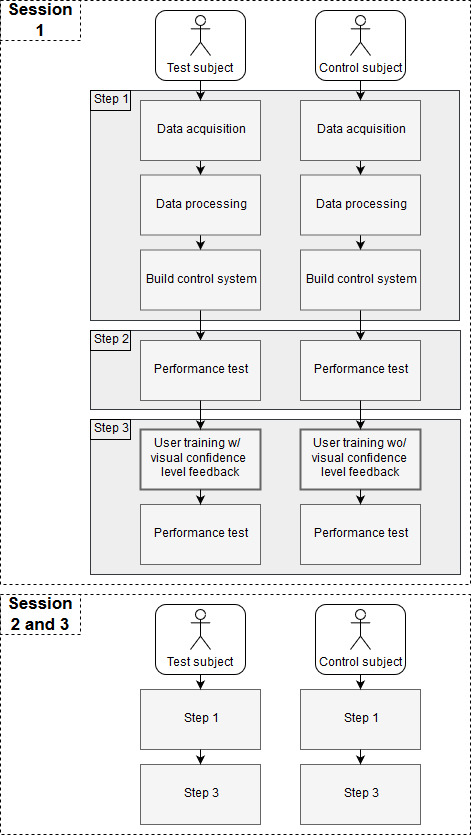
\includegraphics[width=0.64\textwidth]{figures/pMethods/Study_design}  
	\caption{Graphical illustration of the experiment showing the steps of each session for the test and control group. Highlighted is user training in step 3 which is the only procedure that varies between the two groups, and thus the area of research interest in the experiment.}
	\label{fig:std} 
\end{figure}   
